% This is a template for Ph.D. dissertations in the UCI format.

% All fonts, including those for sub- and superscripts, must be 10 points or larger.
% Recommended sizes are 14-point for chapter headings, 12-point for the main body of text
% and figure/table titles, and 10-point for footnotes, sub- and super-scripts, and text in
% figures and tables.
\documentclass[12pt,fleqn]{ucithesis}

\usepackage{amsmath}
\usepackage{array}
\usepackage{bm}
\usepackage{boxedminipage}
\usepackage{graphicx}
\usepackage{natbib}
\usepackage{path}
\usepackage{psfrag}
\usepackage{relsize}
\usepackage{subfigure}

% plainpages=false fixes the "duplicate ignored" error with page counters
% Set pdfborder to 0 0 0 to disable colored borders around PDF hyperlinks
\usepackage[plainpages=false,pdfborder={0 0 0}]{hyperref}

\graphicspath{{figures/}}

% Uncomment the following line to enable Unicode support. This will allow you
% to enter non-ASCII characters (such as accented characters) directly without
% having to use LaTeX's awkward escape syntax (e.g., \'{e})
% NOTE: You may have to install the ucs.sty package for this to work. See:
% http://www.unruh.de/DniQ/latex/unicode/
% \usepackage[utf8x]{inputenc}

\begin{document}

\thesistitle
{
  Improvements to Calico\\
  A sketching application
}

\degreename{Master of Science}

% Use the wording given in the official list of degrees awarded by UCI:
% http://www.rgs.uci.edu/grad/academic/degrees_offered.htm
\degreefield{Informatics}

% Your name as it appears on official UCI records.
\authorname{Mitchell Ryan Dempsey}

% Use the full name of each committee member.
\committeechair{Professor Andr\'{e} van der Hoek}
\othercommitteemembers
{
  Professor James A. Jones\\
  Professor David Redmiles
}

\degreeyear{2012}

\copyrightdeclaration
{
  {\copyright} {\Degreeyear} \Authorname
}

% If you have previously published parts of your manuscript, you must list the
% copyright holders; see Section 3.2 of the UCI Thesis and Dissertation Manual.
% Otherwise, this section may be omitted.
% \prepublishedcopyrightdeclaration
% {
%   Chapter 4 {\copyright} 2003 Springer-Verlag \\
%   Portion of Chapter 5 {\copyright} 1999 John Wiley \& Sons, Inc. \\
%   All other materials {\copyright} {\Degreeyear} \Authorname
% }

% The dedication page is optional.
\dedications
{
  To my parents...
}

\acknowledgments
{
  I would like to thank...

  You must acknowledge grants and other funding assistance. 

  You may also acknowledge the contributions of professors and friends. 
  
  You also need to acknowledge any publishers of your previous work who have given you permission to incorporate that work into your dissertation. See Section 3.2 of the UCI Thesis and Dissertation Manual.
}


\thesisabstract
{
  The text of the abstract begins here. The text may contain a maximum of 350 words. Include a short statement of the problem you studied, a brief exposition of the methods and procedures employed in gathering the data, and a summary of your findings. No graphs, charts, or tables may be included.
}

\preliminarypages

\chapter{Introduction}
% [Sketching in software design]
% [what limits current systems from doing what we do]
% [with respect to the needs we have, they fall short]
% [how does calico overcome those limitations]

Formal design notations are best used for documenting a system, and do not work well when designing. This is the very reason that many designers turn to a whiteboard in order to sketch their designs. A platform that allows for sketching allows the designer to work without any restrictions at all [ON WHAT?] on designers and the drawings they are able to easily create. Designers are then able to freely manipulate their drawings without the burden of a structured design document. The software is able to aid the designer in creation of their drawing, but does not prevent the flexibility that a traditional whiteboard provides.  

When working at the whiteboard, developers typically draw very informal table-napkin type drawings that are used to quickly build a solution to a given problem. Whiteboards are excellent tools for this, as they provide very little resistance to quick sketching. 

The affinity that designers have for using a whiteboard has been recognized across many different disciplines of design. Sketching plays a very crucial, and very universal role in all applications of design. [this seems so weak?]

Current software design tools offer the user a great amount of power when it comes to tool support. Designers can generate diagrams and other documentation artifacts using these tools. However, these tools do not seem to exist when it comes to sketching. Designers need a tool that is flexible and fluid like a whiteboard, but powerful enough to be useful to designers as a tool.  

Calico is a software-sketching tool used by designers to help them easily draft potential software systems. Calico was designed to be used with a multi-touch whiteboard and projector so that it can replicate the role of a traditional whiteboard. We hoped to build upon the ease-of-use that a whiteboard provides designers, but while at the same time providing options and benefits that a traditional whiteboard system lacks. [I feel like I say this over and over] We hope that Calico can be used to be overcome the limitations of a traditional whiteboard, while not suffering the disadvantages of a structured design tool. While using a whiteboard is very fluid and unrestricted, a whiteboard does not provide any help to a designer – it is identical to pen-and-paper drawings. 

Our research has been about designing Calico, which is very similar to a traditional whiteboard in that it allows the user to sketch freely, but does not suffer from all of the disadvantages that a whiteboard does. One advantage Calico has over a traditional whiteboard is collaboration. Being a distributed, networked design system, Calico can enable designers to collaborate with one another across the globe – something that a traditional whiteboard could never achieve. [what do you think is the best “story” to tell here?]

[RANDOM PARA]To improve the existing version of Calico, we decided to vastly improve the architecture in order to natively support collaboration. We had a few requirements that we wanted to satisfy with the new architecture. The first was the need for the system to be distributed. Originally, we wanted to support two boards that were placed next to each other and just provide a link between those two boards. However, in the end we decided against that and chose to create a system that would allow any number of clients, from various locations to interact on the same space. The second requirement was extensibility. We wanted to easily be able to add plugins and new features to Calico. The previous version proved to be very difficult to add new features, so our goal was to solve that problem, and easily allow new things to be added. The final requirement was reliability. We needed to have a system that was able to stay online, and retain the drawings that we created. Old versions of calico would crash, and then all designs would be lost. By having a centralized server, we hope that the server would be able to outlive client crashes and problems, and could be much more stable because it was not handling any graphical interface. With our new architecture we were able to continually experiment with new features. We could see which features were working well, and which ones were rarely used and could then be removed. The relative ease to adding new features made experimenting with new ideas very easy.

\chapter{Background}

To better understand our reasoning for creating Calico, it is useful to have some insight into the history of sketching, and in particular the history of sketching in software design. Designers rely on sketching as part of their own thought process.
% PD Stuff Here
When working collaboratively, designers use whiteboards to sketch design ideas, explore solutions, capture code fragments, decide on division of tasks as well as scheduling tasks. As discussed in\cite{chen1} the key advantages of using whiteboards for sketching include immediacy, versatility, size and collaboration. There is very little effort to access a whiteboard, whiteboards are capable of multiple as well as secondary mutations, the size allows for more than one sketch and finally a whiteboard allows multiple designers to work on and discuss evolving designs. 

Within the design literature several studies have looked at how designers behave when they are tasked with a complex design problem. Four general observations drove the development of Calico. Designers use low detail in sketching designs because the sketches are only initial thoughts and reflections\cite{a8} they are intentionally rought and without detail. Designers frequently shift their focus during intial phases and these original sketches are often revisited at a later time\cite{a9}. Designers often sketch, whether as a concious decision or not, ambiguous designs leaving room for later improvement\cite{a3}. Finally designers use a wide variety of languages when expressing designs whether it might be diagrams or informal symbols\cite{a6}. Calico was designed to aid software designers in creating and manipulating early software designs.
% /PD

Sketching allows designers to express their ideas in a very fluid and flexible manner.
Sketching allows designers to not be hindered by design software that tries to enforce a specific design style. Designers are able to be as meticulous as they wish, and they are not spending time working around the roadblocks created by a structured design system.
It is very easily for a designer to cross out a given idea and then immediately create an alternative. Designers typically work with a visual image in their head\cite{todo}, and sketching provides the least amount of friction when trying to put that visual image into the design.
This flexibility allows them to focus on the formation of ideas and discussion, without having to worry about how the discussion itself is being documented. 
Sketching allows ideas to be more easily viewed, analyzed, and discussed -- much more than would be possible without some representational notation.
Another benefit afforded by sketching is the ability to view a design from a higher-level or ``bird’s-eye view''.
This high-level view allows designers to discover design paths that they would have otherwise overlooked had the idea not been drawn out and understood. 

\todo{ANDRE: How is this unique to sketching versus a design tool?}
Sketching allows designers to create representations of concepts that can be linked together in order to create a very detailed design. For example, flowcharts can be created that show how logic will flow through a program. As another example, database designers can use sketching to informally show foreign key relations when designing a schema. 

Often in sketching, designers are able to mix very different design styles that a normal software design program would not be allow in the same space. As you can see in \todo{Add image}Figure, designers at a local company are creating sketches in order to design a software product. You can see how they have linked various components in the system to each other, so that they can create an overview of how the system will function.

% PD stuff here
The free flowing process of sketching allows for open-ended thought processes during initial phases of design, regardless of discipline. Sketching allows designers to have flexibility while they explore design problems. It allows them to go from abstract thoughts to concrete ideas\cite{todo}. Sketching allows designers to formulate new ideas, combine, transform, and also reject ideas\cite{todo}. In general, sketching allows the designer a path by which they can go from their original thoughts to a more concrete design. During this process, the designer can diverge from his original thoughts and gain insight from the sketching itself\cite{todo}.

Many have studied the value in sketching as the basis of the design process. Zannier found that tools that encouraged conversations between designers gave way to decisions that considered more alternatives\cite{todo}. Cherubini has found that designers use sketching as a way of brainstorming and manipulating concepts\cite{todo}. Software designers often sketch as a natural extension of the thought process used during the design phase to view more than a single solution simultaneously\cite{todo}.

\todo{ANDRE: Too fast, separate sections. 1) background of sketching 2) sketching tools}
Early tools, such as SILK\cite{todo} or DENIM\cite{todo} interpret shapes sketched by a user into model elements. Later tools such as SUMLOU\cite{todo} and Marama-Sketch\cite{todo} left the sketches in their original form until the user requested the translation into a formal diagram. Inkkit\cite{todo} advanced further by supporting multiple levels of formality. Other UML-oriented tools also followed similar design processes\cite{todo}.

While these programs do provide freedom of expression for a user, they still force the diagram into a specific notation. All of these tools focus on what can be sketched.

Early work in the computer-supported cooperative work (CSCW) community looked at how users can work collaboratively. Others have studied the interaction mechanisms and integrating tablet PC based input on a large display for a group of designers to work together\cite{todo}
% / PD


In the context of software design, sketching tools prove to be even more useful. These tools allow designers to create several varying solutions in parallel, and then chose the best of these designs to continue designing. Sketching allows software designers to fluidly move focus between various potential ideas in order to contrast designs with others. Software design tools that do not force a specific design structure on the user can encourage a broader consideration of alternative designs, and can greatly improve the eventual design outcome.

\chapter{Calico}

% [anticpated/actual features]
% [purpose, how does it work]
% [supports designers in sketching]

\section{Canvas and Grid}

\begin{figure}[htb]
\centering
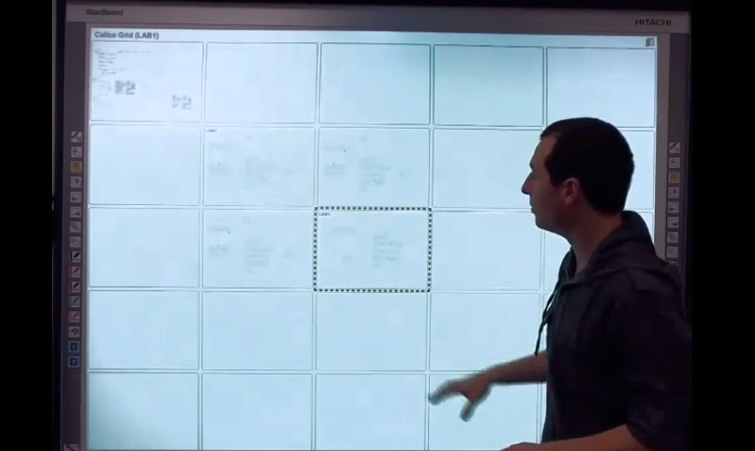
\includegraphics[width=0.8\textwidth]{grid.jpg}
\caption{The grid view within Calico}
\label{fig:grid}
\end{figure}
The grid is the focal point of any session in Calico.
It shows the various canvases that users may interact with in a given session.
Users may perform various operations on canvases from the grid, such as duplicating or clearing individual cells.
The grid also gives a clear overview of the designs that are happening in a session.

\section{Gestures}

\section{Scraps}
Scraps in Calico can be thought of as ``scraps of paper'' that one would place on a desk or on a white board.
Scraps can be easily relocated to different parts of the screen, or even other canvases.
Scraps can be stacked on top of each other and then treated as a unit or group.
By treating scraps as if they were pieces of paper, we [make it easy to understand the manipulation], as designers can easily relate Calico to their current design 

\section{Palette}
The palette in Calico provides users with a ``drawer'' that can easily be used to store commonly used shapes and artifacts.
The palette can be synchronized across sessions so that other users in the session can share the same palette.
\chapter{Objectives}

[old version was single user, list limitations] Calico was originally designed to be a single-user system that allowed individuals to operate an electronic whiteboard. While this original design worked great in an isolated environment, it made it very difficult for users to collaborate with one another. Users had to resort to taking screenshots and emailing them to one another.  Our aim with the new version of Calico was to create a system that would function in an isolated environment, but could easily facilitate collaboration with multiple users when needed. By designing with collaboration in mind, we were able to create a client-server architecture that would support many users interacting with the same canvas area simultaneously. The server had to be responsible for maintaining order of objects, as well as acting as a version control to make sure that users were not able to perform conflicting actions that would corrupt the drawings.

As an experiment, we worked to add collaboration to the original Calico implementation. This was able to help us determine that using Calico in a multi-user environment would be much more useful than we originally expected, and drove us to create a more robust multi-user implementation. Our attempts to [make old calico multi-user] were not successful, as the system was extremely sluggish and frustrated many users. We found that our users expected the system to be much more responsive, and the sluggishness was not acceptable. This was one of the biggest reasons that we decided to redesign a new Calico from the ground up.  

[reasoning for new iteration, rethinking architecture]Rather than continue working on the existing version of Calico, we discussed the [usefulness?] of redesigning the architecture from the ground up in order to better support the features we were hoping to add. We wanted to create a system based on the client-server architecture that would facilitate many clients all interacting with the system at the same time. The old version of Calico used a peer-to-peer connection that limited the number of active clients that could use the system. The old peer-to-peer architecture proved to be highly problematic when connecting with users over the Internet. While the system was able to work fine locally, the ultimate goal for the system was to collaborate with users all over the world, and we realized that a peer-to-peer architecture would not be ideal when collaborating over the Internet. This was one of the reasons we chose to move to a client-server architecture. We were able to place the server on a system that was open to the Internet, and it would eliminate all the connection problems that plagued the old peer-to-peer architecture. 

Another area where the client-server architecture benefitted us was with performance. We created a server that was highly optimized for processing data from many different clients at the same time. This allowed us to handle many more clients without any noticeable drop in processing time. Previous versions of Calico had the clients act as servers, which meant that in addition to processing all of the graphical data, they were also responsible for processing all incoming data and drawing what the other clients were sending.
[list requirements and wants/needs]
[req:distributed]
[req:persistence]The first iteration of Calico was a peer-to-peer system. This meant that there was no single place where the drawings would be stored. There was no way to view the contents of the session unless you were actively viewing it from within the Calico program itself. We wanted to be able to access the current state of a session without the need to actually join the session itself. By creating a central server that was responsible for maintaining the session, we were able to have a persistent history of the session. Users could join and disconnect, and then return, and still be able to undo operations that were performed long ago. Users could import canvas drawings into other programs by requesting a rendered image from the server. By storing the session state at a single location, we reduced the likelihood that data would become corrupted in transit, or data that would be corrupted synchronizing between many "master" servers as it had in the traditional peer-to-peer architecture. The persistent server was regarded as the true master, and if any client differed, it would synchronize with the central server, rather than assuming its own state was the "correct" version.

[req:sessions]Sessions was not initially planned in our rewrite of Calico, but we soon found a need for sessions to be added. The previous version of Calico had no session system at all, however it was not really necessary because users could essentially create their own sessions by just starting another instance of the program. This provided an easy method for users to work on various projects without interfering with the designs of another project. With the new client-server architecture, it was more difficult to start a new instance of the server in order to work on a separate project. Thus the need for sessions was realized, as designers needed a way to easily create a separate Calico instance that would not interfere with the existing session. 

[req:admin interface]One of the benefits of having a central server was the ability to have an "administrative interface" that could allow users to perform actions on the server, and backup/restore sessions. With the new version of Calico, we opted to create a web-based administrative interface that let the user perform various low-level commands that were used for debugging. Along with the ability to perform commands, users could download a file containing the entire state of a session. These files could then be restored at a later point in time, and would restore the session to its previous state. This proved to be very useful during the initial development, as it provided a safety net for users. Users were able to experiment more knowing they had a backup of their designs.

\chapter{High-Level Architecture}
% high level architecture
% how accomplish objectives from above
% what changes, rationale
% how it actually works
% checksums/persistence/how model is updated
% dealing with parallel edits
% updating clients
% presence awareness
% 1) architecture  (why) [distributed/reliable/multiple boards]
% 2) "new htink" - why
% design decisions
% new archi
% experience with it

\chapter{Implementation?}
\chapter{Related Work}
%[what have other sketching tools done so far]
%[are there other distributed tools that do similar things]
%[what have we borrowed ideas from]

\chapter{Conclusion}
In conclusion, Calico is awesome.


% These commands fix an odd problem in which the bibliography line
% of the Table of Contents shows the wrong page number.
\clearpage
\phantomsection

\bibliographystyle{abbrv}
\bibliography{thesis}

%\appendix
%\section{Appendix A}

\end{document}
